\documentclass[conference]{IEEEtran}
\usepackage[utf8]{inputenc}
\usepackage{graphicx}
\usepackage{listings}
\graphicspath{{images/}}

\begin{document}

\title{Tarea 4: Procesamiento de Grafos}
\author
{\IEEEauthorblockN{Alberto Pascal Garza}
\IEEEauthorblockA{Análisis y Diseño de Algoritmos\\
\\Profesor Vicente Cubells\\
ITESM Campus Santa Fe\\
C.P: 01389\\
Email: A01023607@itesm.mx}
}
\maketitle

\begin{abstract}
En este reporte de investigación se hablará sobre la exportación de grafos a distintos formatos para así poder ser representados visualmente en programas como gephi. Este procedimiento es nos facilita el entendimiento de nuestro grafo dado a que se puede ver gráficamente la relación entre los distintos nodos . Además, se analizará el proceso contrario. Es decir, se analizará la forma en que podemos importar los contenidos de nuestros grafos a un archivo de texto para su utilización y manipulación en otros formatos.Es necesario hacer uso de la biblioteca de Snap-4.0
\end{abstract}

\section{Introducción}
Los grafos son una estructura de datos compuesta por una serie de nodos, vértices y aristas. Son ampliamente utilizados para representar información. Es una de las formas más versátiles de ver información gráfica dado que se puede representar con cualquier tipo de estructuras (es decir, pilas, colas, árboles). Algunas de sus aplicaciones van desde tomar decisiones en videojuegos, las relaciones entre las amistades de usuarios de redes sociales o cualquier otro tipo de redes. Además,  podemos utilizar métodos de búsqueda y de exploración tales como Prim, Kruskal, Bellman Ford, Floyd Warshall, BFS, DFS y Dijkstra para hacer de su uso más eficiente.

\section{Metodología}
Para realizar la actividad se generó un código capaz de leer de un archivo de texto un grafo con una gran cantidad de nodos. Para poder hacer esto, se utilizó la librería de Snap-4.0 (obtenida de Standford Network Analysis Project). Además, dicho código se modificó para poder exportar el grafo leído a los formatos GraphML, GEXF, GDF y JSON Graph Format. De esta forma, se pudieron utilizar los archivos exportados al programa Gephi, el cual es cpaz de representar gráficamente nuestros datos y poder obtener información más relevante.

\subsection{Procedimiento}
\subsubsection{Descargar la información del grafo (dataset)}
Para obtener la información del grafo que se empleó en esta actividad se descargó de  la página oficial de la universidad de Stanford (https://snap.stanford.edu/data/index.html.) un dataset que contuviera la información en  formato ".txt". De esta forma se podrá implementar en el código fuente de conversión.

\subsubsection{Implementación de las funciones en C++}
Para poder hacer uso de las funciones se instaló previamente la librería de SNAP. Para hacer esto, se descargó el arhcivo de la librería y se escribió dentro de la terminal el comando "make all". El código del programa se escribió usando el lenguaje C++. Fue necesaro poner el código dentro de la carpeta de SNAP para poder hacer uso de "stdafx.h", que permite la utilización de las funciones para cargar el grafo (LoadEdgeListo). Además, se hizo uso del objeto "pUNGraph" que permite utilizar iteradores para escribir parista por arista el archivo de salida en todos los formatos antes mencionados.

\subsubsection{Importación del grafo exportado a Gephi}
Una vez que nuestro grafo fue exportado mediante la ejecución de nuestro código fuente es necesario importarl a la herramienta Gephi. De esta forma, Gephi podrá representar gráficamente a nuestro grafo. Para esta actividad se utilizó el dataset que contenía los mensajes de texto mandados dentro de una red social de la  Irvin, en California. A continuación se muestra su representación gráfica:
\ 
\\  

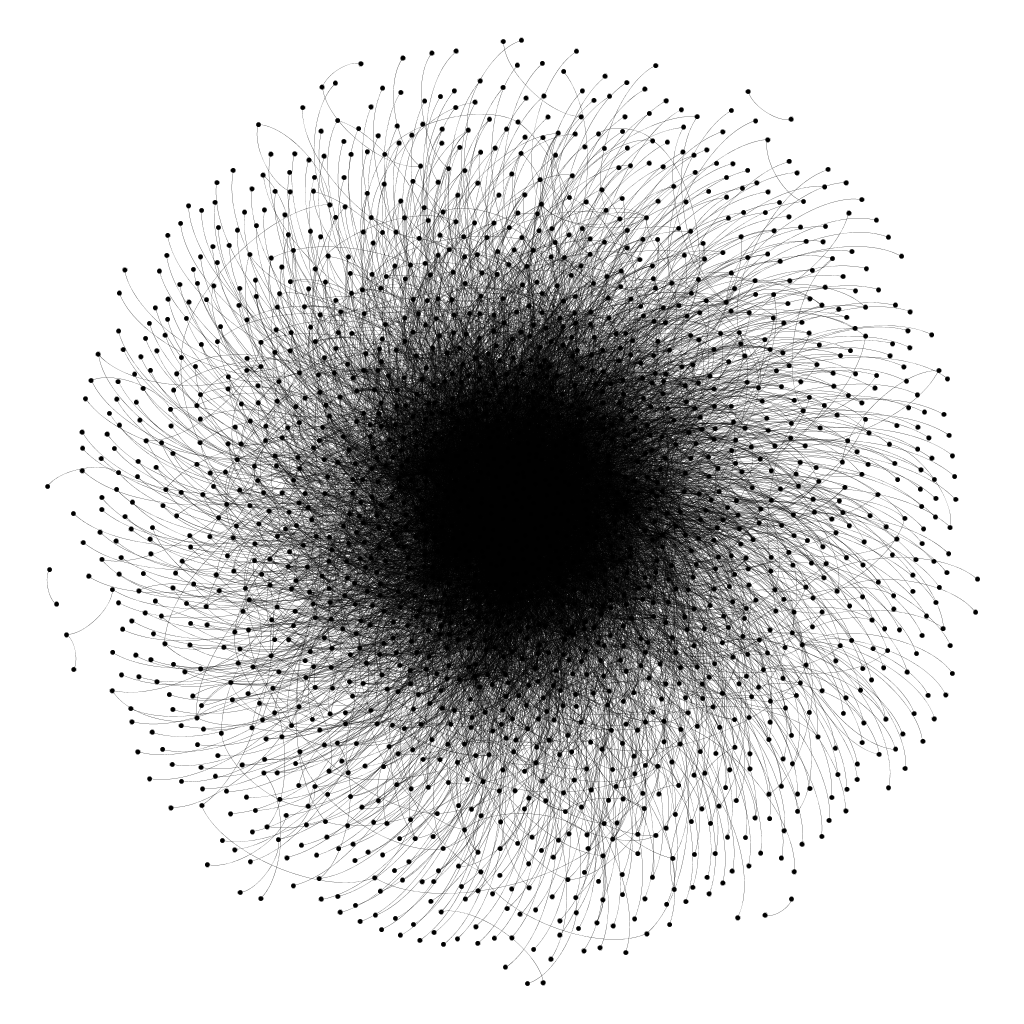
\includegraphics[width=\linewidth]{grafo}
\ 

\section{Ventajas y desventajas de los formatos}
Los visualizadores de grafos nos permiten tener una mejor claridad de nuestro grafo para poder analizarlo con mayor precisión. Sin embargo, de todos los formatos en los que podemos existen algunos que nos proporcionan más privilegios que otros. Como tal no existe un mejor formato para todas las situaciones sino que debemos adaptarnos según los requisitos que se nos presenten. Es importante mencionar que sólamente GraphML, GDF y GEXF pueden reconocer las posiciones, colores y tamaño de todos los atributos. Lamentablemente, aunque éstos últimos tres son de los más usados, presentan distintas funcionalidades entre sí. GraphML es el que nos permite detallar más la información. GEXF nos permite definir en un espaico temporal los valores de nuestro grafo y GDF tiene la ventaja de ser el más ligero de los formatos. En cuanto a sus desventajas,  tanto GraphML como GEXF son de los formatos más pesados debido a la cantidad de información y detalle que manejan por lo que en algunos dispositivos pueden ser problemáticos. GDF es el más ligero de todos pero presenta la desventaja de no tener tanto detalle como los dos anteriores. Por esto mismo, existe una cuarta opción llamada JSON, la cuál nos permite balancear la simpleza de la información con el redimiento del grafo para utilizarlo en cualquier dispositivo.


\subsection{GraphML}
GraphML está hecho a partir de una estructura de XML. Por esto mismo, tiene una ventaja en cuanto a lo versátil que puede ser al momento de intercambiar datos del grafo entre plataformas. Además, es el formato estándar más legible y relativamente sencillo de entender. Posee la capacidad para representar los grafos tales como sus pesos y cada una de sus aristas que, además, representa mediante el uso de distintos colores, tamaños y posición. Nos provee de la capacidad de crear grafos con jerarquías y establecer valores predetermindados para los atributos específicos de los nodos y aristas.
\subsection{GEXF}
Así como GraphML, GEXF se basa en la estructura XML para así poder tener más versatilidad de transferencia de datos. GEXF  tiene todas las capacidades de GraphML, pero cuenta con la ventaja adicional de darle un tiempo de vida especifico a cada nodo, arista o atributo. De esta manera se puede definir en qué momento en el tiempo se deben de alterar los valores o simplemente eliminarse un nodo o arista específico haciendo de este formato ideal para proyectos más dinámicos. La manera en que se implementa esta capacidad es mediante dos formas, un atributo de tipo "double" o con el formato internacional de fecha y hora (yyyy-mm-dd).


\subsection{GDF}
GDF es un formato más ligero y , por lo tanto,  cuenta con una menor complejidad espacial. Se utiliza para la creación de grafos y a diferencia de los formatos anteriores, solo almacena la información necesaria que pudiese necesitar un grafo con atributos tales como pesos en las aristas, atributos para los nodos/aristas, atributos de visualización y la posibilidad de establecer valores predeterminados. Por lo tanto carece de funcionalidades interesantes como el tiempo de vida de los nodos/aristas/atributos y la posibilidad de hacer grafos con jerarquías.

\subsection{JSON Graph Format}
JSON, que es en realidad JavaScript Object Notation, es un formato para intercambiar datos. Es una de las alternativas a XML. Utiliza JavaScript y puede ser leido por cualquier lenguaje de programación. Por esto mismo, JSON puede ser utilizado para el intercambio de información entre distintas tecnologías. Es un formato simple que genera archivos de menor tamaño y posee una velocidad de procesamiento alta aunque su estructura es difícil de interpretar a simple vista. Debido a esto, es ideal para dispositivos con menores prestaciones como los teléfonos móviles en donde la duración de la batería y el consumo de datos es un factor muy importante.

\section{Complejidad temporal y espacial de cada función}

\subsection{Exportación a GraphML}
\begin{itemize}
\item Complejidad temporal: O(N+A) (N=Nodos, A=Aristas)
\item Complejidad espacial: S(1)
\item Tiempo de ejecución: 15 ms
\end{itemize}

\subsection{Exportación a GEXF}
\begin{itemize}
\item Complejidad temporal: O(N+A)
\item Complejidad espacial: S(1)
\item Tiempo de ejecución: 21 ms
\end{itemize}

\subsection{Exportación a GDF}
\begin{itemize}
\item Complejidad temporal: O(N+A)
\item Complejidad espacial: S(1)
\item Tiempo de ejecución: 7 ms
\end{itemize}

\subsection{Exportación a JSON}
\begin{itemize}
\item Complejidad temporal: O(N+A)
\item Complejidad espacial: S(1)
\item Tiempo de ejecución: 11 ms
\end{itemize}


\begin{thebibliography}{9}
\bibitem{JSONvsXML}
Oscar Blancarte
\textit{JSON vs XML}.
recuperado el 22 de octubre de 2017 de: https://www.oscarblancarteblog.com/2014/07/18/json-vs-xml/

\bibitem{Learning to Discover Social Circles in Ego Networks}
J. McAuley and J. Leskovec
\textit{Learning to Discover Social Circles in Ego Networks}
recuperado el 22 de Octubre de 2017 de:  NIPS, 2012\

\bibitem{JSON}
Alejandro Esquiva
\textit{¿Qué es y para qué sirve JSON?}
recuperado el 22 de octubre de 2017 de: https://geekytheory.com/json-i-que-es-y-para-que-sirve-json/

\bibitem{Gephi1}
Gephi
\textit{Supported Graph Formats}
recuperado el 22 de octubre de 2017 de: https://gephi.org/users/supported-graph-formats/

\bibitem{Gephi2}
Gephi
\textit{GEXF File Format}
recuperado el 22 de octubre de 2017 de: https://gephi.org/gexf/format/dynamics.html

\bibitem{Gephi3}
Gephi
\textit{GraphML}
recuperado el 22 de octubre de 2017 de: https://gephi.org/users/supported-graph-formats/graphml-format/

\bibitem{Gephi4}
Gephi
\textit{GDF Format}
recuperado el 22 de octubre de 2017 de: https://gephi.org/users/supported-graph-formats/gdf-format/
\end{thebibliography}

\appendix
\section{Repositorio de GitHub}
https://github.com/AlbertoPascal/Tarea4\_algoritmos

\onecolumn
\newpage
\section{Código empleado}


\lstinputlisting[language=C++, basicstyle=\tiny]{prueba.cpp}

\end{document}
